\subsubsection{Convection using a pressure--temperature look-up table and the rheology of Steinberger and Calderwood (2006)}
\label{sec:cookbooks-steinberger}

\textit{This section was contributed by Juliane Dannberg and Ren{\'e} Gassm{\"o}ller.}

In this cookbook we will go one step further from the last one and set up a fully compressible mantle convection model using the projected density approximation (where the density is interpolated onto the finite element grid to compute the density gradients in the mass conservation equation rather than approximating these gradients using a reference profile or temperature/pressure derivatives of the density, see \cite{gassmoller2020formulations}). To compute the material properties, we read in a look-up table of material properties in dependence of temperature and pressure, originally computed using a mineral physics software (in this case, Perple\_X, \cite{connolly2005computation}). The table is based on the thermodynamic database of \cite{stixrude2011thermodynamics} and a pyrolitic composition \cite{ringwood1988nature}. Compared to a 1D profile, a temperature-pressure look-up table has the advantage that material properties are accurate not only around one reference adiabat, but also for strongly deviating pressures and temperatures. This is particularly important at phase transitions, because their depth depends on the temperature and pressure.

This cookbook also demonstrates how to read in a viscosity profile from a data file. Specifically, we use the profile and lateral viscosity variations due to temperature from \cite{stca06}, which are based on mineral physics constraints and surface observations. 

In addition, this cookbook shows the use of periodic boundary conditions. 

\paragraph{Geometry and periodic boundaries.}
The model setup is a quarter spherical shell with periodic side boundaries. The inner and outer radius are 3481~\si{\km} and 6371~\si{\km}, respectively, so that the mantle is 2900~\si{\km} deep. In the same section of the input file, we also need to specify that the model should have periodic boundaries in angular ($\phi$) direction:
\lstinputlisting[language=prmfile]{cookbooks/steinberger/doc/geometry.part.prm.out}
Both the top and bottom boundaries allow for free slip. Because the model has periodic side boundary conditions and free slip boundaries at top and bottom, the amount of rigid-body rotation in $\phi$ direction is not constrained. In other words: There is no unique solution. \aspect{} can remove this nullspace from the model (see Section~\ref{sec:nullspace}). Here, we do this by setting the net rotation to zero:
\lstinputlisting[language=prmfile]{cookbooks/steinberger/doc/nullspace.part.prm.out}
The temperature is fixed to 273~\si{\K} at the top and 3773~\si{\K} at the bottom boundary.
The initial temperature model consists of an adiabatic profile,
thermal boundary layers at the surface and the core-mantle boundary, 
and a small harmonic perturbation to initiate convection.
The gravity profile in the model is based on PREM. 

\paragraph{The equation of state.}
To use material properties from a temperature--pressure look-up table, we use the Steinberger material model. We have to specify the path to the directory where all the data files we want to use for this model are stored. This includes the files for the viscosity profile, the lateral viscosity variations due to temperature, and all material files containing look-up tables computed by mineral physics software.
In addition we have to specify the names of these files. 
In our case, we only have one of these look-up tables, because we only have one composition: pyrolite. 
But in principle, the material model can use several compositions with one look-up table for each. 
For intermediate composition values, material properties will then be averaged based on the mass/volume fractions of the individual compositions. 

In addition, there are a few options we can select about how these look-up tables should be used:
We can decide between interpolating between data points in the lookup table based on the pressure and temperature at the point we need the material properties for, or we can simply take the value from the table that is closest. In our case, we choose the bilinear interpolation because it is more accurate. 
Second, we can decide how latent heat should be computed: from the thermal expansivity and specific heat, 
or from the enthalpy (all three properties should be columns in the look-up table). 
In some cases the look-up table contains the effective thermal expansivity and specific heat. Using these effective properties automatically includes the latent heat release and consumption at phase transformations in the adiabatic heating term and the left-hand side term (change in thermal energy over time) of the energy equation. In a case like that, we simply want to use these values without using additional latent heat terms because latent heat is already included automatically when using the properties from the look-up table. 
If the look-up table contains thermal expansivity and specific heat without the effect of phase transitions, then \aspect{} can compute latent heat effects based on the pressure and 
temperature derivatives of the specific enthalpy (using the approach of \cite{nakagawa2009incorporating}).
In our case, we simply do not include latent heat at all in our model.
So the look-up table is computed without latent heat effects, and we set the ``Latent heat'' parameter to \texttt{false}.
\lstinputlisting[language=prmfile]{cookbooks/steinberger/doc/lookup.part.prm.out}
In an actual research application, it would be appropriate (and consistent with the projected density approximation, or any other compressible approximation) to compute latent heat instead of neglecting it as we do. This often leads to numerical instabilities that one typically addresses by ensuring that either the resolution is fine enough so that each phase transitions is resolved by several mesh cells,
or the energy equations needs to be solved for entropy instead of pressure (which is an option available in \aspect{}; in this case, the look-up table needs to be given in terms of entropy and pressure). 

\paragraph{The look-up table format.}
The format of these look-up tables is described in the documentation of the \href{https://aspect.geodynamics.org/doc/doxygen/classaspect_1_1MaterialModel_1_1MaterialUtilities_1_1Lookup_1_1MaterialLookup.html}{aspect::MaterialModel::MaterialUtilities::Lookup::MaterialLookup} class.
Two different formats are currently supported: Perple\_X and HeFESTo. 
The format needs to be selected in the input file, and each format has a specific header and needs to be structured in a specific way. The paragraph below explains how to structure a Perple\_X file. 
This file format is the default, it is also the more flexible format and it is what is used in this cookbook. Since the only requirements for the format are the header and the order of some of the columns, 
files created with other mineral physics software can also be converted to this format.  

The Perple\_X header contains the following in the first 13 lines: 
\begin{enumerate}
  \item The Perple\_X version,
  \item the name of the data table,
  \item the dimensions of the data table (for example, for a table with one dimension being pressure, the other temperature, this would be 2),
  \item the variable in the first dimension (this either needs to be \texttt{T(K)} for temperature, or \texttt{P(bar)} for pressure),
  \item the minimum value of this variable,
  \item the increments this variable will be increased with in the table,
  \item the number of different values of this variable the table contains,
  \item the second variable,
  \item the minimum value of this second variable,
  \item the increments this second variable will be increased with in the table,
  \item the number of different values of this second variable the table contains,
  \item the number of material properties in the table, and finally,
  \item the names of the columns.
\end{enumerate}
The first two columns need to be the pressure and temperature (in any order). The other required column names are:
\texttt{rho,kg/m3} (for the density), \texttt{alpha,1/K} (for the thermal expansivity), \texttt{cp,J/K/kg} (for the specific heat), \texttt{vp,km/s} (for the P-wave velocity), \texttt{vs,km/s} (for the S-wave velocity)), \texttt{h,J/kg} (for the specific enthalpy).
Optionally, the file can contain columns with the name \texttt{phase} (to read in the name of the dominant phase), and columns named \texttt{vol\_fraction\_} and the name of a phase after the second underscore (to read in volume fractions of different phases).
As an example, the header of the table used in this cookbook is given below:

\begin{lstlisting}
|6.6.6
PYR-Ringwood88_2.tab                                                                                
           2
T(K)    
   400.00360000000001     
   19.999960000020000     
         181
P(bar)  
   15001.334999999999     
   5114.9322988556905     
         262
           8
T(K)           P(bar)         rho,kg/m3      alpha,1/K      cp,J/K/kg      vp,km/s        vs,km/s        h,J/kg 
\end{lstlisting}

Below this header, the table contains the actual data values, using one column for each of the property names given in the last line of the header. 
It is also useful to know that \aspect{} does not actually read in the values of the pressures and temperatures in the first two columns, but instead uses the minimum, increment, and number of values parameters given in the header, assuming a uniform step size. The first column is always assumed to be the inner loop (i.e., it needs to increase first while the second column stays constant). 




\paragraph{The rheology.}
The rheology of this model consists of two parts: The viscosity profile, and the lateral variations due to temperature. For each of these, we need to read in a data file. In this example, we use files that are based on \cite{stca06} for both. The viscosity profile is based on mineral physics and surface constrains, and the lateral viscosity variations use an Arrhenius law with a depth-dependent activation enthalpy. For more details and a derivation, see \cite{stca06}. 

Other rheology models can be used by reading in different files. The formatting of these files is the following: The radial viscosity file contains two columns, where the first is the viscosity in \si{\pascal\second}, and the second is the depth in \si{\km} (note that this is an exception to the usual \aspect{} convention of using SI units). The lateral viscosity file also contains two columns, the first being the activation enthalpy divided by the gas constant and the nondimensional stress exponent (which is 1 for diffusion creep/in the lower mantle, and 3.5 for dislocation creep/in the upper mantle and transition zone in the model of \cite{stca06}). The second column is depth, again in \si{\km}. 
Both parts are combined to compute the viscosity in the following way:
\begin{equation}
  \eta = \eta_\text{rad} \exp{ \left( -\frac{V_\text{lat} \Delta T}{T T_\text{ref}} \right)} , 
\end{equation}
where $\eta_\text{rad}$ is the value from the radial viscosity file, 
$V_\text{lat}$ is the value from the lateral viscosity file, 
$T$ is temperature, $T_\text{ref}$ is the reference temperature profile, 
and $\Delta T$ is the deviation from the reference temperature profile. 

This reference profile can be chosen in two different ways: On the one hand, it can be chosen as the laterally averaged temperature (and in this case, a number of depth slices for this lateral averaging can be specified as  well). This is the original formulation of \cite{stca06}, and the default of the material model. 
On the other hand, the adiabatic temperature profile can be chosen as the reference. 
However, the radial profile needs to be adapted based on how this reference temperature is chosen. 
If the reference profile uses the laterally averaged temperature, then the radial profile needs to include a high viscosity in the lithosphere (where it is cold), and a low viscosity near the core-mantle boundary (where it is warm). If the reference profile is the adiabatic profile, then the temperature will deviate from this reference in the top and bottom thermal boundary layers already, leading to changes in viscosity. So in this case, the radial profile should not include these boundary layers (because otherwise we would compute their effect twice). This option allows the viscosity in the boundary layers to develop based on the temperature in the model, which is why we choose it for this cookbook. 

The default data directory already contains two radial viscosity files, one for each of these cases. 
The file \url{data/material-model/steinberger/radial-visc.txt} is the original Steinberger and Calderwood \cite{stca06} profile (with an interpolation between the original discrete layers) and for use with the laterally averaged temperature. The file \url{data/material-model/steinberger/radial-visc-simple.txt} is for use with the adiabatic profile. To illustrate the difference, the content of both files is plotted in Figure~\ref{fig:steinberger-viscosity}. 

\begin{figure}
  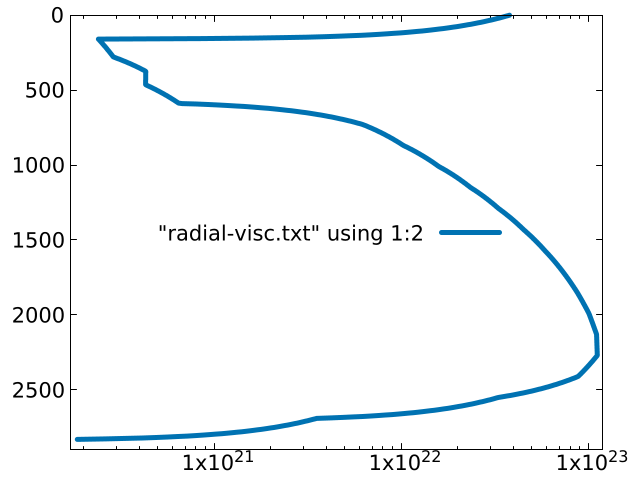
\includegraphics[width=0.48\textwidth]{cookbooks/steinberger/doc/radial-visc.pdf}
  \includegraphics[width=0.48\textwidth]{cookbooks/steinberger/doc/radial-visc-simple.pdf}
  \caption{\it Left: Viscosity profile based on the original \cite{stca06} formulation, intended for use with a temperature-dependence of viscosity based on the laterally averaged temperature. Right: Modified viscosity profile without boundary layers, intended for use with a temperature-dependence of viscosity based on an adiabatic temperature profile.}
  \label{fig:steinberger-viscosity}
\end{figure}

In order to improve solver convergence, the material model has additional parameters that allow it to limit the viscosity variations. 
Because of the resolution in this cookbook we limit the lateral viscosity variations to 
three orders of magnitude in both directions (for a total of six orders of
magnitude), and we additionally limit the overall viscosity
between $10^{20}$~\si{\pascal\second} and $5 \times 10^{23}$~\si{\pascal\second}. This allows the features of the flow field to be resolved. 
\lstinputlisting[language=prmfile]{cookbooks/steinberger/doc/rheology.part.prm.out}
In the Earth, we would expect higher viscosities in the lithosphere and 
lower viscosities in plumes and near the core-mantle boundaries. 
This type of viscosity formulation is appropriate for global convection models. 
However, it does not approximate lithospheric deformation well. 
The model only accounts for diffusion creep, so the 
lithosphere has a high viscosity and forms a stagnant lid on top of the 
sublithospheric mantle. In order to achieve more realistic subduction in a model like this, 
one would have to either prescribe plate velocities at the surface 
(forcing plates to subduct) or take into account plastic yielding (so that
the lithosphere can break).

\note{If the model takes too long to run, increase the minimum viscosity.}

\paragraph{The projected density approximation.}
Since our model is compressible, the most accurate way to solve the mass 
conservation equation implemented in \aspect{} is to use the `projected density
approximation'. This way, \aspect{} will compute the density gradients in the 
mass conservation directly from the density field (interpolated onto the 
finite element grid) rather than approximating it with a reference profile 
or temperature/pressure derivatives of the density. 

To use the projected density approximation, we need to specify it as the form of the equations we want to use, and we need to provide a field that the density values can be interpolated on. 
The first part is handled in the `Formulation' section of the input file. This is where we can select 
the projected density approximation as the formulation we want to use for the mass conservation equation. 
The temperature equation uses the real density (rather than a reference profile) as well. 

To allow for the interpolation, we create a compositional field that we call `density\_field'. 
We assign the field the type `density', so that \aspect{} knows that this is the field it should use to compute the density gradient required to solve the equations. \aspect{} does not need to solve an 
equation for this field, it only needs to interpolate the density values onto it. 
This is covered by the compositional field method `prescribed field'. 
For fields of this type, the material model provides the values that should be 
interpolated onto the field.
\lstinputlisting[language=prmfile]{cookbooks/steinberger/doc/projected_density.part.prm.out}

The complete input file can be found in \url{cookbooks/steinberger/doc/steinberger.prm}. 

\paragraph{Results.} We run the model for 300 million years. Over the time of the model evolution, some plumes rise and spread beneath the base of the lithosphere, and some cold downwellings detach from the base of the lithosphere. The temperature at the end of the model run and some of the material properties are shown in Figure~\ref{fig:steinberger-end-state}. 

\begin{figure}
  \includegraphics[width=0.48\textwidth]{cookbooks/steinberger/doc/temperature.png}
  \includegraphics[width=0.48\textwidth]{cookbooks/steinberger/doc/viscosity.png}
  \includegraphics[width=0.48\textwidth]{cookbooks/steinberger/doc/density.png}
  \includegraphics[width=0.48\textwidth]{cookbooks/steinberger/doc/specific_heat.png}
  \caption{\it End state of the model. From left to right and top to bottom: Temperature, viscosity, density, and specific heat capacity.}
  \label{fig:steinberger-end-state}
\end{figure}

